\documentclass{beamer}

% --- packages
\usepackage[utf8]{inputenc}
\usepackage[spanish]{babel}

\usepackage{hyperref}

\usepackage{bm}

\usepackage{nicematrix}

\usepackage{stanli}

\usepackage{listings}
\lstset{
  breaklines=true,
}
\usepackage{dirtree}

\usepackage[style=apa,citestyle=apa]{biblatex}
% \DefineBibliographyStrings{spanish}{%
%   andothers = {et al}
%   }
\addbibresource{bibliografia.bib}
% ---

% --- tema
\usetheme{Madrid}
% ---

% --- Portada
\title[Cuaterniones en pyFEM] %optional
{Aplicación de los cuaterniones en el análisis matricial}

\subtitle{Implementación de pyFEM}

\author[Ramirez, Estrada] % (optional, for multiple authors)
{Cristian Ramirez \and Martín Estrada}

\institute[UNAL] % (optional)
{
  Facultad de ingeniería\\
  Universidad Nacional de Colombia
}

\date[INDETEC 2020] % (optional)
{IX seminario permanente de divulgación de resultados de investigación grupo INDETEC, Noviembre de 2020}

\logo{
\includegraphics[height=1.5cm]{escudo_unal.png}}
% ---

\begin{document}

\begin{frame}
  \titlepage
\end{frame}

% \section*{Outline}
\begin{frame}
  \frametitle{Tabla de contenido}
  \tableofcontents
\end{frame}

\section{Introducción}
\begin{frame}
  \frametitle{Introducción}
  \begin{block}{Definición}
    pyFEM: programa de computador para el análisis de estructuras en tres dimensiones tipo pórtico sometidas a cargas estáticas.    
  \end{block}

  \begin{columns}
    \column{0.5\textwidth}
    \dirtree{%
      .1 pyFEM.
      .2 pyFEM.
      .3 classtools.py.
      .3 core.py.
      .3 primitives.py.
      .2 test.
      .3 space\_frame.py.
      .3 trusses.py.
      .2 LICENSE.
      .3 README.md.
    }
    \column{0.5\textwidth}
    \href{https://github.com/rvcristiand/pyFEM}{github.com/rvcristiand/pyFEM}
  \end{columns}
\end{frame}

\begin{frame}
  \frametitle{Introducción}
  \begin{block}{Definción}
    FEM.js: programa de computador para visualizar estructuras tridimensionales.
  \end{block}
  \begin{columns}
    \column{0.5\textwidth}
    \begin{figure}
      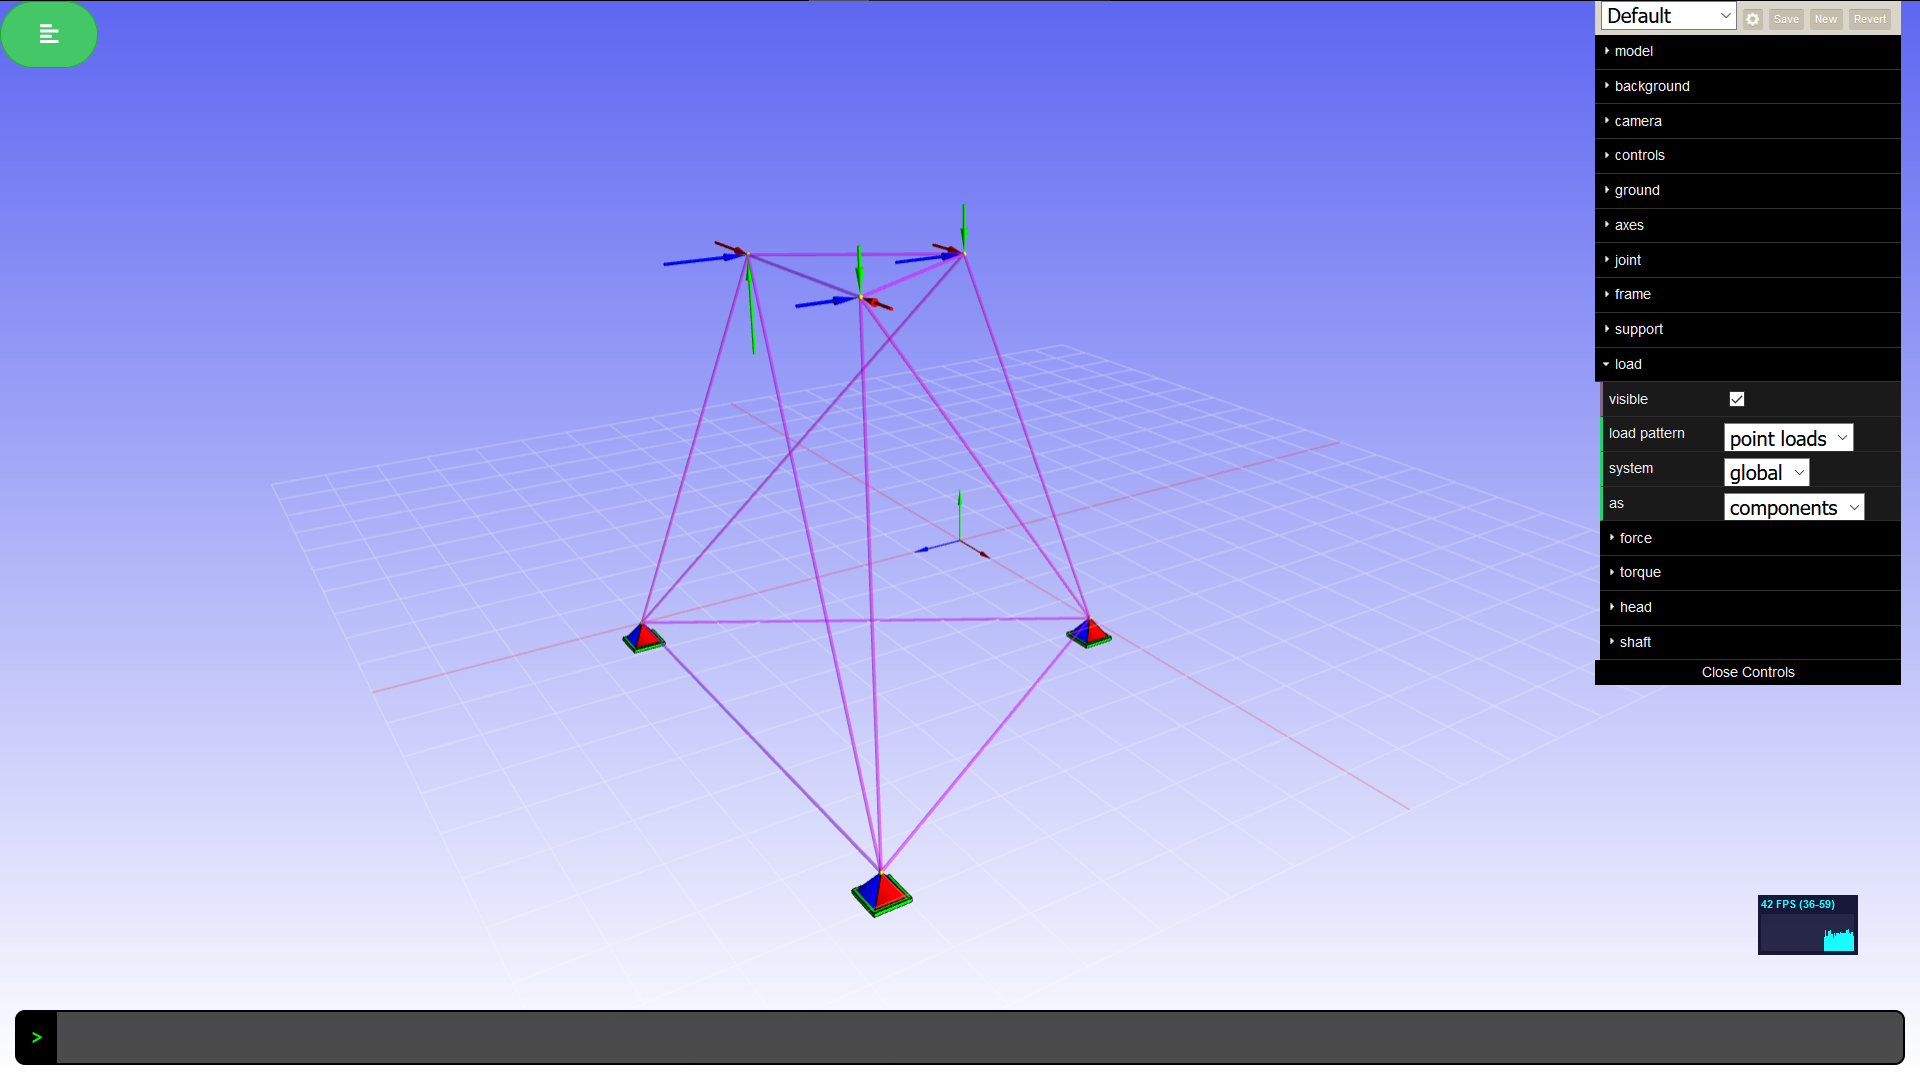
\includegraphics[width=1\textwidth]{FEM.js.png}
      \caption{FEM.js ejecutandose en el navegador de internet.}
    \end{figure}
    \column{0.5\textwidth}
    \href{https://github.com/rvcristiand/FEM.js}{github.com/rvcristiand/FEM.js} \\
    
    \href{https://rvcristiand.github.io/FEM.js}{rvcristiand.github.io/FEM.js}
  \end{columns}
\end{frame}

\section{pyFEM}
\begin{frame}
  \frametitle{pyFEM}
  \framesubtitle{Elemento tipo pórtico}
  \begin{figure}
    \centering
    \begin{tikzpicture}[coords]
      % points
      \dpoint{a}{0}{0}{0};
      \dpoint{b}{4}{0}{0};

      \dpoint{alabel}{0}{0}{0.25};
      \dpoint{blabel}{4}{0}{0.25};

      \dpoint{beamlabel}{2}{0}{0.25};

      \dpoint{jux}{-1}{0}{0};
      \dpoint{juy}{0}{-1.5}{0.25};   
      \dpoint{juz}{0}{0}{-1.25};

      \dpoint{jrx}{-2}{0}{0};
      \dpoint{jry}{0}{-2.75}{0.25};   
      \dpoint{jrz}{0}{0}{-2.5};

      \dpoint{kux}{4.5}{0}{0};
      \dpoint{kuy}{4}{-1.5}{0.25};   
      \dpoint{kuz}{4}{0}{-1.25};

      \dpoint{krx}{5.25}{0}{0};
      \dpoint{kry}{4}{-2.75}{0.35};   
      \dpoint{krz}{4}{0}{-2.5};   
      
      % beams
      \dbeam{1}{a}{b};

      \dnotation{6}{beamlabel}{\emph{i}};

      % supports
      \dsupport{2}{a}[yz];
      \dsupport{2}{b}[yz];

      \dnotation{1}{alabel}{\emph{j}};
      \dnotation{1}{blabel}{\emph{k}};
      % restrains
      % j
      \dload{1}{a}[270][0][1];
      \dload{1}{a}[270][90][1][0.5];   
      \dload{1}{a}[180][180][1][0.5];

      \dload{3}{a}[270][0][1][1.25];
      \dload{3}{a}[270][90][1][1.75];   
      \dload{3}{a}[180][180][1][1.75];

      \dnotation{1}{jux}{1};
      \dnotation{1}{juy}{2};
      \dnotation{1}{juz}{3};

      \dnotation{1}{jrx}{4};
      \dnotation{1}{jry}{5};
      \dnotation{1}{jrz}{6};   
      
      % k
      \dload{2}{b}[90][0][1];
      \dload{1}{b}[270][90][1][0.5];   
      \dload{1}{b}[180][180][1][0.5];

      \dload{4}{b}[90][0][1][1.25];
      \dload{3}{b}[270][90][1][1.75];   
      \dload{3}{b}[180][180][1][1.75];

      \dnotation{1}{kux}{7};
      \dnotation{1}{kuy}{8};
      \dnotation{1}{kuz}{9};

      \dnotation{1}{krx}{10};
      \dnotation{1}{kry}{11};
      \dnotation{1}{krz}{12};
      
      % axes
      \dscaling{3}{1};
      \daxis{1}{0, 0, 0};
    \end{tikzpicture}
    \caption{Elemento tipo pórtico en coordenadas locales.}
    \label{fig:space-frame}
  \end{figure}
\end{frame}

\begin{frame}
  \frametitle{pyFEM}
  \framesubtitle{Matriz de rigidez}
  \begin{equation}
    \begin{bNiceArray}{CCCCCCCCCCCC}[small,
      first-row,
      first-col,
      code-for-first-row = \mathbf{\arabic{jCol}},
      code-for-first-col = \mathbf{\arabic{iRow}}
      ]
      
      & & & & & & & & & & & & \\
      & \frac{EA_x}{L} & 0 & 0 & 0 & 0 & 0 & -\frac{EA_x}{L} & 0 & 0 & 0 & 0 & 0 \\
      & & \frac{12EI_z}{L^3} & 0 & 0 & 0 & \frac{6EI_z}{L ^2} & 0 & -\frac{12EI_z}{L^3} & 0 & 0 & 0 & \frac{6EI_z}{L^2} \\
      & & & \frac{12EI_y}{L^3} & 0 & -\frac{6EI_y}{L^2} & 0 & 0 & 0 & -\frac{12EI_y}{L^3} & 0 & -\frac{6EI_y}{L^2} & 0 \\
      & & & & \frac{GI_x}{L} & 0 & 0 & 0 & 0 & 0 & -\frac{GI_x}{L} & 0 & 0 \\
      & & & & & \frac{4EI_y}{L} & 0 & 0 & 0 & \frac{6EI_y}{L^2} & 0 & \frac{2EI_y}{L} & 0 \\
      & & & & & & \frac{4EI_z}{L} & 0 & -\frac{6EI_z}{L^2} & 0 & 0 & 0 & \frac{2EI_z}{L} \\
      & & & & & & & \frac{EA_x}{L} & 0 & 0 & 0 & 0 & 0 \\
      & & & & & & & & \frac{12EI_z}{L^3} & 0 & 0 & 0 & -\frac{6EI_z}{L^2} \\
      & & & & & & & & & \frac{12EI_y}{L^3} & 0 & \frac{6EI_y}{L^2} & 0 \\
      & & & & & & & & & & \frac{GI_x}{L} & 0 & 0 \\
      & & & & & & & & & & & \frac{4EI_y}{L} & 0 \\
      & \text{sim.} & & & & & & & & & & & \frac{4EI_z}{L}
      \label{eq:matriz-rigidez-elemento-portico}
    \end{bNiceArray}
  \end{equation}
\end{frame}

\begin{frame}
  \frametitle{pyFEM}
  \framesubtitle{Teorema de rotación de Euler}
  \begin{columns}
    \column{0.5\textwidth}
    \begin{block}{Definición}
      Según el \emph{teorema de rotación de Euler} (véase \cite{euler_rotations}), siempre es posible encontrar un diámetro de una esfera cuya posición es la misma después de rotarla alredor de su centro, por lo que cualquier secuencia de rotaciones de un sistema coordenado tridimensional es equivalente a una única rotación alrededor de un eje que pase por el origen.\\
    \end{block}

    \column{0.5\textwidth}
    \begin{figure}
      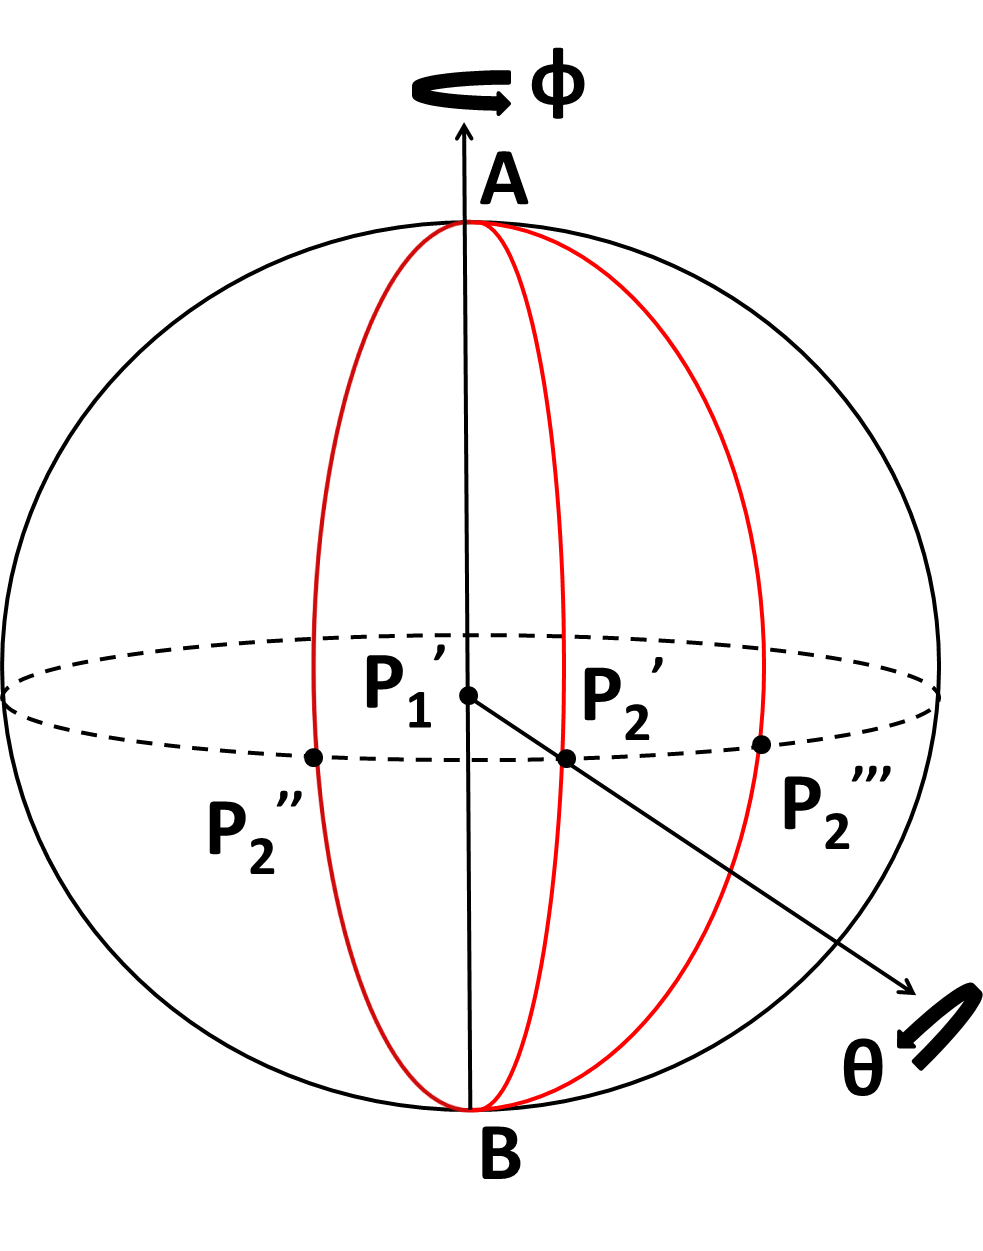
\includegraphics[width=0.5\textwidth]{euler_rotation.png}
    \end{figure}
  \end{columns}      
\end{frame}

\begin{frame}
  \frametitle{pyFEM}
  \framesubtitle{Rotación del sistema de coordenadas}
  \begin{columns}
    \column{0.5\textwidth}
    El ángulo $ \theta $ y el vector $ n $  que definen la rotación del eje $ x $ del sistema de coordenadas global hacia el eje $ x_m $ del sistema de coordenadas de un elemento se puede calcular como
    \begin{equation}
      \begin{aligned}
        \mathbf{n} &= (1, 0, 0) \times \mathbf{x_m} \\
        \theta &= \arcsen((1, 0, 0) \cdot \mathbf{x_m})
      \end{aligned}
    \end{equation}
    \column{0.5\textwidth}
    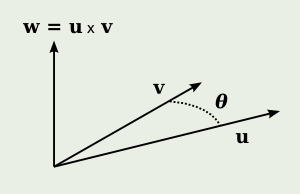
\includegraphics{quaternion_two_vectors.png}
  \end{columns}
\end{frame}

\begin{frame}
  \frametitle{pyFEM}
  \framesubtitle{Representación de la rotación como un cuaternión}
  Según \cite{dunn20023d}, la rotación de un sistema de coordenadas tridimensionales alrededor del eje $ \boldsymbol{n} $ una cantidad $ \boldsymbol{\theta} $ se puede describir mediante un \emph{cuaternión} como
  \begin{equation}
    \boldsymbol{q} =
    \begin{bmatrix}
      cos(\theta/2) & sin(\theta/2) \boldsymbol{n}
    \end{bmatrix} =
    \begin{bmatrix}
      w & x & y & z
    \end{bmatrix}
  \end{equation}
  y se puede obtener la matriz de rotación a partir de un cuaternión de la siguiente manera
  \begin{equation}
    \mathbf{R} =
    \begin{bNiceMatrix}
      1 - 2y^2-2z^2 & 2xy + 2wz & 2xz - 2wy \\
      2xy - 2wz & 1 - 2x^2-2z^2 & 2yz + 2wx \\
      2xz + 2wy & 2yz-2wx & 1 - 2x^2 - 2y^2
    \end{bNiceMatrix}
  \end{equation}
\end{frame}

\section{Implementación de los cuaterniones}
\begin{frame}[fragile]
  \frametitle{Implementación de los cuaterniones}

  \begin{lstlisting}[language=Python]
    class Frame(AttrDisplay, metaclass=UniqueInstances):
        __slots__ = ('joint_j', 'joint_k', 'material', 'section')

        def __init__(self, joint_j=None, joint_k=None, material=None, section=None):
            self.joint_j = joint_j
            self.joint_k = joint_k
            self.material = material
            self.section = section
  \end{lstlisting}
\end{frame}

\begin{frame}[fragile]
  \frametitle{Implementación de los cuaterniones}

  \begin{lstlisting}[language=Python]
    class Frame(AttrDisplay, metaclass=UniqueInstances):
        def get_length(self):
            return distance.euclidean(self.joint_j.get_coordinate(), self.joint_k.get_coordinate())

        def get_direction_cosines(self):
            vector = self.joint_k.get_coordinate() - self.joint_j.get_coordinate()

            return vector / linalg.norm(vector)
  \end{lstlisting}
\end{frame}

\begin{frame}[fragile]
  \frametitle{Implementación de los cuaterniones}
 
  \begin{lstlisting}[language=Python]
    def get_rotation(self):
        v_from = np.array([1, 0, 0])
        v_to = self.get_direction_cosines()
        if np.all(v_from == v_to):
            return Rotation.from_quat([0, 0, 0, 1])
        elif np.all(v_from == -v_to):
            return Rotation.from_quat([0, 0, 1, 0])
        else:
            w = np.cross(v_from, v_to)
            w = w / linalg.norm(w)
            theta = np.arccos(np.dot(v_from, v_to))
            return Rotation.from_quat([x * np.sin(theta/2) for x in w] +
                   [np.cos(theta/2)])
  \end{lstlisting}
\end{frame}

\section{Conclusiones}
\begin{frame}
  \frametitle{Conclusiones}
  Durante el ejercicio de la profesión como ingenieros civiles es habitual que usemos diferentes programas comerciales para el análisis y diseño de estructuras, con la imposibilidad de saber exactamente que rutinas siguen para llegar a los resultados que nos presentan. \\[2ex]

  La intención con este trabajo es dar el primer paso para crear una herramienta a \emph{código abierto} para permitirle a los ingenieros depurar el programa para constatar que los cálculos realizados por el programa son los correctos.
\end{frame}

\section{Bibliografía}
\begin{frame}
  \frametitle{Bibliografía}
  \printbibliography
\end{frame}

\begin{frame}
  \centering \Large
  \emph{Gracias}
\end{frame}
\end{document}